\section{Caracterização e Preparação dos Dados}
\label{sec:caracterizacao}

\subsection{Harmonização e qualidade}
\label{sec:qualidade}

Todas as séries foram levadas à mesma convenção: o instante $t$ indica o início da hora, no horário de Brasília. A carga verificada, publicada em intervalos de 30~minutos em UTC, foi convertida e agregada pela média, de modo que o valor em MW médios da hora equivale à energia em MWh. Na reanálise, as variáveis instantâneas (temperatura e vento) foram associadas à hora pela média dos seus dois extremos, e a irradiância, que já é uma média horária, foi apenas deslocada.

O subsistema Nordeste do ONS corresponde a oito estados (AL, BA, CE, PB, PE, PI, RN e SE). O clima é amostrado em \NPontosClima{} pontos: as oito capitais, ponderadas pela população, para a carga; 16~polos eólicos e 10~solares, obtidos por \textit{k-means} sobre as coordenadas das usinas do SIGA, com peso proporcional à potência (Figura~\ref{fig:mapa}). As usinas com dados horários somam \NEol{} conjuntos eólicos (\CapEolConj~GW) e \NSol{} solares (\CapSolConj~GW).

\begin{figure}[htb]
\centering
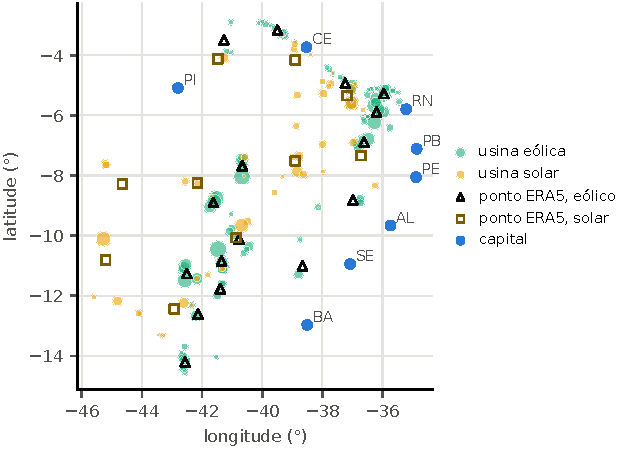
\includegraphics{fig_mapa}
\caption{Usinas eólicas e solares com dados horários no ONS e pontos da reanálise ERA5.}
\label{fig:mapa}
\end{figure}

Não foram encontradas duplicatas nem lacunas internas nas séries centrais, e nenhum valor foi imputado. O balanço do ONS fecha em todas as horas de 2022 a 2025. Entre janeiro e maio de 2026 há \HorasNaoFecha{} horas em que ele não fecha, provavelmente por ainda estar em consistência, e essas horas foram excluídas das comparações com 2026. Três problemas exigiram uma decisão de método e são tratados a seguir: a mudança de definição da carga, o efeito dos cortes sobre a geração e o número reduzido de anos observados.

\subsection{Carga e geração distribuída}
\label{sec:carga}

Em 29/04/2023, o balanço do ONS passou a incluir a micro e minigeração distribuída (MMGD) estimada, tanto na carga quanto na geração solar. Isso produz um degrau de cerca de 0,5~GW na carga (Figura~\ref{fig:carga}) que não corresponde a aumento de consumo. Por isso, a carga modelada vem da série de carga verificada, que informa separadamente a carga global e a MMGD com a mesma definição desde 2022. As duas são modeladas em separado: a forma da carga líquida muda de um ano para outro, à medida que a MMGD reduz o consumo do meio-dia, enquanto a da carga global é mais estável.

\begin{figure}[htb]
\centering
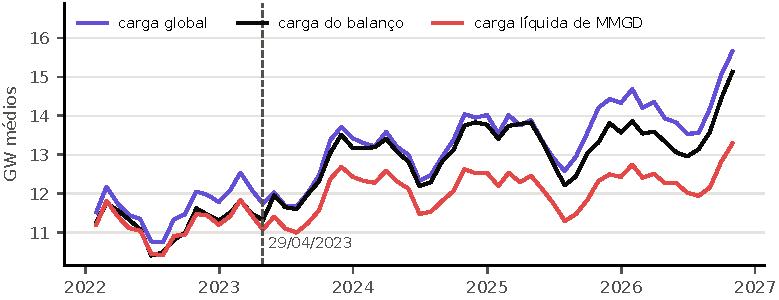
\includegraphics{fig_carga}
\caption{Carga média mensal do Nordeste em três definições.}
\label{fig:carga}
\end{figure}

A carga diária cresce cerca de \CargaGrau\% por grau Celsius (correlação de \CorrTempCarga{} nos dias úteis) e fica \CargaFds\% menor nos fins de semana e feriados. A Figura~\ref{fig:perfis} mostra os perfis por hora e mês. A carga líquida é mínima ao meio-dia e máxima entre 18 e 22~horas. A eólica é mais forte à noite e entre julho e outubro, e a solar só produz de dia. No início da noite, a solar já cessou e a eólica ainda não atingiu o seu máximo.

\begin{figure}[htb]
\centering
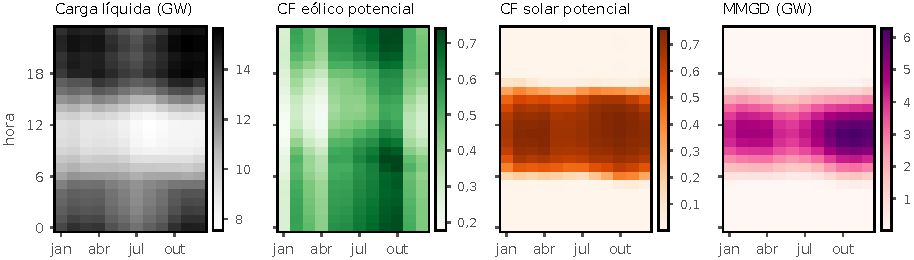
\includegraphics{fig_perfis}
\caption{Perfis médios por hora do dia e mês em 2025.}
\label{fig:perfis}
\end{figure}

\subsection{Geração eólica e cortes}
\label{sec:cortes}

O fator de capacidade (CF) é a razão entre a geração e a capacidade das mesmas usinas na mesma hora. A geração observada, porém, já desconta os cortes, que passaram de \CorteIni\% do potencial em 2022 para \CorteTres\% em 2023, \CorteQuatro\% em 2024 e \CorteCinco\% em 2025 (\CorteTWh~TWh). Com isso, a correlação entre o cubo do vento e o CF observado caiu de \CorrObsIni{} em 2022 para \CorrObsFim{} em 2025 (Figura~\ref{fig:cfvento}).

O alvo adotado é o CF potencial, dado pela soma da geração com a energia cortada apurada pelo ONS, dividida pela capacidade. Com ele, a correlação com o cubo do vento permanece entre \CorrPotMin{} e \CorrPotMax{} em todos os anos. A geração de referência, também publicada pelo ONS, não foi usada como potencial porque fica abaixo da geração verificada em \RefAbaixo\% das horas-usina.

\begin{figure}[htb]
\centering
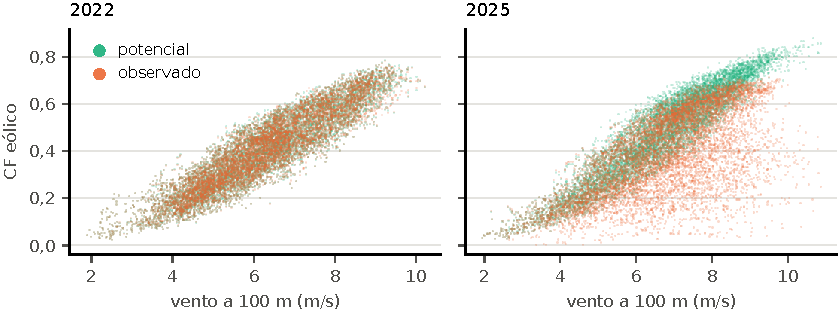
\includegraphics{fig_cf_vento}
\caption{Fator de capacidade eólico observado e potencial em função do vento a 100~m, em 2022 e 2025.}
\label{fig:cfvento}
\end{figure}

\subsection{Anos de clima}
\label{sec:anosclima}

Os quatro anos com dados completos do ONS são, em média, pouco ventosos. Estimado para a frota atual em cada ano da reanálise, o CF eólico varia de \CfMin{} (2009) a \CfMax{} (2012). Entre 31~anos, 2022 é o quarto menos ventoso, 2024 o sétimo, 2023 o décimo primeiro e 2025 o vigésimo terceiro, e a média de 2022 a 2025 é \CfQuatro, contra \CfTrintaUm{} nos 31~anos. Usar somente esses quatro anos levaria a uma estimativa enviesada da geração e não incluiria os anos extremos.
